\documentclass[english, 11 pt, class=article, crop=false]{standalone}
%\documentclass[english, 11 pt]{report}
\usepackage[T1]{fontenc}
\usepackage[utf8]{luainputenc}
\usepackage{babel}
\usepackage[hidelinks, bookmarks]{hyperref}
\usepackage{geometry}
\geometry{verbose,tmargin=1cm,bmargin=3cm,lmargin=4cm,rmargin=4cm,headheight=3cm,headsep=1cm,footskip=1cm}
\setlength{\parindent}{0bp}
\usepackage{amsmath}
\usepackage{amssymb}
\usepackage{esint}
\usepackage{import}
\usepackage[subpreambles=false]{standalone}
%\makeatletter
\addto\captionsenglish{\renewcommand{\chaptername}{Kapittel}}
\makeatother
\usepackage{tocloft}
\addto\captionsenglish{\renewcommand{\contentsname}{Innhold}}
\usepackage{graphicx}
\usepackage{placeins}
\raggedbottom
\usepackage{calc}
\usepackage{cancel}
\makeatletter
\usepackage{color}
\definecolor{shadecolor}{rgb}{0.105469, 0.613281, 1}
\usepackage{framed}
\usepackage{wrapfig}
\usepackage{bm}
\usepackage{ntheorem}

\usepackage{ragged2e}
\RaggedRight
\raggedbottom
\frenchspacing

\newcounter{lign}[section]
\newenvironment{lign}[1][]{\Large \refstepcounter{lign} \large
	\textbf{\thelign #1} \rmfamily}{\par\medskip}
\numberwithin{lign}{section}
\numberwithin{equation}{section}
\usepackage{xcolor}
\usepackage{icomma}
\usepackage{mathtools}
\usepackage{lmodern} % load a font with all the characters
\usepackage{xr-hyper}
\makeatother
\usepackage[many]{tcolorbox}

%\setlength{\parskip}{\medskipamount}
\newcommand{\parskiplength}{11pt}
%\setlength{\parskip}{0 pt}
\newcommand\eks[2][]{\begin{tcolorbox}[enhanced jigsaw,boxrule=0.3 mm, arc=0mm,breakable,colback=green!30] {\large \textbf{Eksempel #1} \vspace{\parskiplength}\\} #2 \vspace{1pt} \end{tcolorbox}\vspace{1pt}}

\newcommand\fref[2][]{\hyperref[#2]{\textsl{Figur \ref*{#2}#1}}}
\newcommand{\hr}[2]{\hyperref[#2]{\color{blue}\textsl{#1}}}

\newcommand\rgg[2][]{\begin{tcolorbox}[boxrule=0.3 mm, arc=0mm,colback=orange!55] #2 \vspace{1pt} \end{tcolorbox}\vspace{-2pt}}
\newcommand\alg[1]{\begin{align*} #1 \end{align*}}
\newcommand\algv[1]{\vspace{-11 pt} \begin{align*} #1 \end{align*}}
\newcommand\vs{\vspace{-11 pt}}
\newcommand\g[1]{\begin{center} {\tt #1}  \end{center}}
\newcommand\gv[1]{\begin{center} \vspace{-22 pt} {\tt #1} \vspace{-11 pt} \end{center}}
%\addto\captionsenglish{\renewcommand{\contentsname}{Løsningsforslag tentamen R2 H2015}}

% Farger
\colorlet{shadecolor}{blue!30} 

% Figur
\usepackage{float}
\usepackage{subfig}
\captionsetup[subfigure]{labelformat=empty}
\usepackage{esvect}

\newcommand\sv{\textbf{Svar:} \vspace{5 pt} \\}

%Tableofconents
\renewcommand{\cfttoctitlefont}{\Large\bfseries}
\setlength{\cftsubsecindent}{2 cm}
\newcommand\tocskip{6 pt}
\setlength{\cftaftertoctitleskip}{30 pt}
\setlength{\cftbeforesecskip}{\tocskip}
%\setlength{\cftbeforesubsecskip}{\tocskip}

%Footnote:
\usepackage[bottom, hang, flushmargin]{footmisc}
\usepackage{perpage} 
\MakePerPage{footnote}
\addtolength{\footnotesep}{2mm}
\renewcommand{\thefootnote}{\arabic{footnote}}
\renewcommand\footnoterule{\rule{\linewidth}{0.4pt}}

%asin, atan, acos
\DeclareMathOperator{\atan}{atan}
\DeclareMathOperator{\acos}{acos}
\DeclareMathOperator{\asin}{asin}

%Tabell
\addto\captionsenglish{\renewcommand{\tablename}{Figur}}

% Figur
\usepackage[font=footnotesize,labelfont=sl]{caption}
\addto\captionsenglish{\renewcommand{\figurename}{Figur}}

% Figurer
\newcommand\scr[1]{/home/sindre/R/scr/#1}
\newcommand\asym[1]{/home/sindre/R/asymptote/#1}

%Toc for seksjoner
\newcommand\tsec[1]{\phantomsection\addcontentsline{toc}{section}{#1}
	\section*{#1}}
%\newcommand\tssec[1]{\subsection*{#1}\addcontentsline{toc}{subsection}{#1}}
\newcommand\tssec[1]{\subsection*{#1}}
% GeoGebra
\newcommand{\cms}[2]{{\tt #1( #2 )}}
\newcommand{\cm}[2]{{\large \tt #1( #2 )} \gvs \\}
\newcommand{\cmc}[2]{{\large \tt #1( #2 )} \large (CAS)  \gvs \\ \normalsize}
\newcommand{\cmk}[2]{{\large \tt #1( #2 )} \large (Inntastingsfelt)  \gvs \\ \normalsize}

\newcommand\gvs{\vspace{11 pt}}

\newcommand\vsk{\vspace{11 pt}}
\newcommand{\merk}{\vsk \textsl{Merk}: }
\newcommand{\fig}[1]{
\begin{figure}
	\centering
	\includegraphics[scale=0.5]{fig/#1}
\end{figure}
}
\newcommand{\figc}[1]{
		\centering
		\includegraphics[scale=0.5]{fig/#1}
}

% Opg
%\newcommand{\opgt}{\phantomsection \addcontentsline{toc}{section}{Oppgaver} \section*{Oppgaver for kapittel \thechapter}}
\newcounter{opg}
\numberwithin{opg}{section}

\newcommand{\opl}[1]{\vspace{15pt} \refstepcounter{opg} \textbf{\theopg} \vspace{2 pt} \label{#1} \\}



\begin{document}
\eqlen	
\opgt
\setcounter{section}{1}	
\opl{parlinjeo}
Ei linje går gjennom punktene $ A=(-2, 3, -5) $ og $ B=(-1, 1, -4) $.\os

\textbf{a)}	Finn en parameterframstilling for linja.\os

\textbf{b)} Sjekk om punktene $ C=(-4, 7, -7) $ og $ D=(-3, 5, 4) $ ligger på linja.

\opl{krysslinj}
To linjer $ l $ og $ m $ krysser hverandre i et punkt $ A $. Parameteriseringen til linjene er gitt som
\[l: \left\lbrace{
	\begin{array}{l}
	x=-3-2t  \\
	y= 3+ 2t   \\
	z= 1-t 
	\end{array}
}\right. \quad 
m: \left\lbrace{
	\begin{array}{l}
	x=-7 +3s  \\
	y= 5- 2s   \\
	z= s 
	\end{array}
}\right. \]
Finn koordinatene til $ A $.

\opl{finnparplan}
Et plan inneholder punktene $ (1, 1,-1) $, $ (-2, -3, -1) $ og $ (5, 6, 1) $. \os

\textbf{a)} Finn en parameterisering for planet.\os

\textbf{b)} Sjekk om punktet $ (-9, 5, 3) $ ligger i planet.


\opl{finnparplan2}
Et plan har retningsvektoren $ [2, 1, -5] $ og inneholder linja gitt ved parameteriseringen
\[ l: \left\lbrace{
	\begin{array}{l}
	x=2-4t  \\
	y= -3+ 2t   \\
	z= 5+t 
	\end{array}
}\right. \]


\nes
\opl{finnplan}
Et plan er utspent av vektorene $ [-4, 2, 0] $ og $ [-3, 0, 3] $ og inneholder punket $ (-2, 2, 1) $. Finn en ligning for planet.
\newpage
\opl{finnplan2}
Et plan $ \alpha $ er gitt ved parameteriseringen
\[\alpha: \left\lbrace{
	\begin{array}{l}
	x=-4 + 2s  \\
	y= 2+ 3s + 2t   \\
	z= 1-t 
	\end{array}
}\right. \]
\textbf{a)} Finn to retningsvektorer for planet.\os

\textbf{b)} Finn en ligning for planet.

\opl{finnplan3}
Et plan er gitt ved ligningen
\[ 10x-3y-4z=0 \]
\textbf{a)} Sjekk om punktene $ (1, -2, 4) $ og $ (4, -2, 1) $ ligger i planet.\os

\textbf{b)} Finn en parameterframstilling for planet.

\opl{finnplan4}
Et plan går gjennom origo og inneholder punktet $ A=(-2, 1, 1) $. For en gitt $ t $ er vektoren $ \vec{u}=[3t, 5, t] $ ortogonal med vektoren mellom origo og $ A $. For dette valget av $ t $ er $ \vec{u} $ også en normalvektor for planet. Finn en ligning for planet.

\opl{kuleopg}
Ei kule er gitt ved ligningen
\[ x^2 + 2 x + y^2 - 4 y + z^2 - 12 z + 32 = 0  \]
\textbf{a)} Finn sentrum og radiusen til kula.\os

\textbf{b)} Vis at punktet $ A=(1, 3, 8) $ ligger på kuleflaten.\os

\textbf{c)} Bestem ligningen til tangentplanet til kuleflaten i punktet $ A $. 

\opl{kuleopg2}
Ei kule er gitt ved ligningen 
\[ x^2 - 6x + y^2 + 2y + z^2 - 10z-14=0 \]
\textbf{a)} Finn sentrum $ S $ og radiusen $ r $ til kula.\os

\textbf{b)} Sjekk om punktene $ A= (4, 1, 6) $ og $ B=(-6, -4, 1) $ ligger innenfor, utenfor eller på kuleflaten.
\newpage
\nes
\opl{avstplinopg} Ei linje $ l $ går gjennom punktene $ (1, 0, -2) $ og $ (2, -2,0) $. Finn avstanden mellom $ l $ og punktet $ (1, -3, 1) $. 

\opl{avstplopg}
Et plan er gitt ved ligningen:
\[ -3x+4y+z-7 = 0 \]
Finn avstanden mellom planet og punktet $ (-3,2,3) $.

\opl{toparllin} 
To parallelle plan $ \alpha $ og $ \beta $ er henholdsvis gitt ved ligningene 
\[ 3x -2y +z +12 = 0 \]
og 
\[ 3x -2y +z = 0  \]
\textbf{a)} Finn en normalvektor til planene.\os

\textbf{b)} Finn et punkt som ligger i ett av planene. \os

\textsl{Hint}: Velg fritt en verdi for $ x $ og $ y $, og løs resulterende ligning for $ z $.\os

\textbf{c)} Finn avstanden mellom planene.\os

\textbf{d)} Finn en parameterframstilling for ett av planene.
\newpage
\opl{kuleopg3}
Når et plan $ \alpha $ skjærer en kuleflate med sentrum $ S $, kan vi alltids studere geometrien fra en slik vinkel at planet ligger rett horisontalt. Et snitt av figuren vil da se slik ut:
\begin{figure}
	\centering
	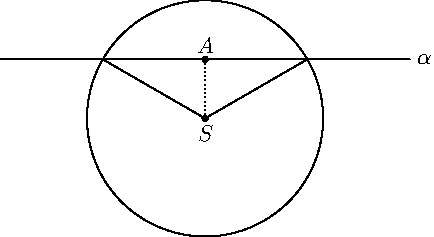
\includegraphics[]{../../asymptote/plkul}
\end{figure}
Punktet $ A $ er sentrum i sirkelen hvor kuleflaten skjærer planet, og ved formlikhet kan vi vise (prøv selv!) at linjestykket $ AS $ står normalt på $ \alpha $.\os

La $ \alpha $ være gitt ved ligningen 
\[ 2x - y - 2z +1=0   \] 
Dette planet skjærer en kuleflate gitt ved ligningen
\[x^2 - 6x + y^2 + 4y + z^2 -23 = \]
\textbf{a)} Hva er avstanden mellom planet og $ S $?\os

\textbf{b)} Finn en parameterframstilling for linja som går gjennom $ A $ og $ S $.\os

\textbf{c)} Finn koordiantene til de to punktene hvor kuleflaten og linja gjennom $ AS $ krysser.\os

\textbf{d)} Hva er koordinatene til $ A $?\os

\textbf{e)} Hvor stor er radiusen til sirkelen hvor $ A $ er sentrum?
\newpage
\ekspop
Vi skal her jobbe oss fram til å vise formelen for avstanden mellom et punkt og et plan (ligning (\ref{avplp})).\vs
\begin{figure}[H]
	\centering
	\subfloat[\textsl{a)}]{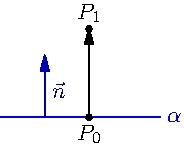
\includegraphics[]{../../asymptote/pktplan}}
	\qquad\quad	
	\subfloat[\textsl{b)}]{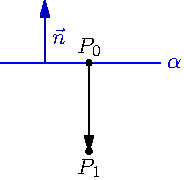
\includegraphics[]{../../asymptote/pktplanb}}	
\end{figure}
På figurene over ser vi skissen av et plan $ \alpha $ som er gitt ved ligningen $ ax+by+cz+d=0 $. Planet inneholder punktet $ P_0=(x_0, y_0, z_0) $ og har en normalvektor $ \vec{n} $. Utenfor planet ligger et punt ${ P_1=(x_1, y_1, z_1) }$, $ P_0 $ er valgt slik at $ {\vv{P_0P_1}\parallel\vec{n}} $.\vsk

\textbf{a)} Forklar hvorfor $ P_0 $ oppfyller ligningen
\[ d=-(ax_0+by_0+cz_0) \tag{I}\label{do} \]
\textbf{b)} Vis at vektoren $ \vv{P_0P_1} $ er gitt som:
\[ \vv{P_0P_1} = [x_1-x_0, y_1-y_0, z_1-z_0] \tag{II}\label{PPo} \]
\textbf{d)} Vis at:
\[ \vv{P_0P_1}\cdot q\vec{n} = \left|\vv{P_0P_1}\right||\vec{n}|\cos \theta  \]kan skrives som:
\[ ax_1+by_1+cz_1+d= \left|\vv{P_0P_1}\right||\vec{n}|\cos \theta \tag{III} \label{skalo} \]
\textsl{Hint}: Bruk (\ref{PPo}) og (\ref{do}).\os

\textbf{f)} Bruk (\ref{skalo}) til å finne formelen for avstanden mellom $ P_1 $ og $ \alpha $.
\end{document}